\documentclass{article}
\usepackage{log_2022}
\usepackage{booktabs}
\usepackage{multirow}
\usepackage{amsfonts}
\usepackage{graphicx}
\usepackage{float}
\usepackage[numbers,compress,sort]{natbib}
\usepackage{xcolor}

\title[Geometric Bias in Flow-Based Protein Structure Generation]{How Does Geometric Bias Shape the Denoising Trajectory\\
in Flow-Based Protein Structure Generation?}
\author[S. Ravishankar]{Shreyas Ravishankar\thanks{Code available at \url{https://github.com/rs-gh/proteina-interpretability}}\\
\institute{University of Cambridge}\\
\email{sr2173@cam.ac.uk}}

\begin{document}
\maketitle

% ============================================================
\begin{abstract}
Proteina is a flow-based generative model for protein backbone structure where geometry enters only as an additive pair bias $B$ to attention scores.
We study two questions in unconditional generation: \emph{when} does $B$ become causally essential during generation, and \emph{where} in the network is it most critical?
Our central finding, in response to the \emph{when} question, is that geometric guidance is memoryless: $B$'s effect depends only on its current availability, not its history. Providing $B$ only during late generation always preserves valid structures, though with gradually reduced quality as the late window shrinks, while providing $B$ only during early generation is indistinguishable from never having $B$ at all.
This temporal asymmetry is universal across all model scales (60M--400M parameters), model architectures, and protein lengths tested, despite order-of-magnitude variation in the descriptive geometry--content balance across models.
However, architecture does change \emph{where} geometry matters: without triangle updates, shallow layers are most sensitive to $B$ removal; with triangle updates, this inverts, and deep layers become critical while shallow layers become dispensable.
Our characterisation motivates future work on representation alignment in generative models for biochemistry.
\end{abstract}

% ============================================================
\section{Introduction}

Generative models for protein backbone structure have advanced rapidly, with flow matching emerging as a leading paradigm~\citep{lipman2023flow}.
Proteina~\citep{geffner2025proteina} scales flow-based protein generation to state-of-the-art quality by combining a transformer backbone with a \emph{pair bias attention} mechanism that fuses learned content scores with geometric pair biases.
Unlike SE(3)-equivariant networks~\citep{thomas2018tensor,fuchs2020se3} or invariant point attention~\citep{jumper2021alphafold2}, Proteina uses standard (non-equivariant) transformer layers, with geometry entering only through an additive pair bias $B$ derived from pairwise distances and sequence separation --- a soft invariant prior that reflects a broader trend toward soft geometric priors over hard-coded symmetries~\citep{dosovitskiy2021image,kim2022tokengt,abramson2024alphafold3}.

We ask two questions about the dynamics of $B$ during unconditional generation: \textbf{when} does geometric bias become causally essential, and \textbf{where} in the network does it act?
Proteina samples via SDE integration from pure noise ($t{=}0$) to a structured backbone ($t{=}1$).
At each step, every attention layer computes:
\begin{equation}
    A = \mathrm{softmax}(C + B)
    \label{eq:attention}
\end{equation}
where $C = QK^\top / \sqrt{d}$ is the content score and $B$ is the pair bias, constructed from binned pairwise distances of the current noisy structure $\mathbf{x}_t$.
At $t{=}0$, these distances are uninformative; at $t{=}1$, they encode the near-final structure.
Since softmax is a nonlinear operation, attribution of $B$'s contribution to $A$ is ambiguous: its effect depends on how $B$ interacts with $C$, not on its magnitude alone. We therefore use four complementary lenses to study $B$'s role, using \emph{early/late} for generation time and \emph{shallow/deep} for layer depth (formalised in Section~\ref{sec:methods}):
\begin{enumerate}
    \item \textbf{Descriptive:} How large is $B$ relative to $C$ in the pre-softmax scores?
    \item \textbf{Causal:} When and where is $B$ necessary for valid structures?
    \item \textbf{Functional:} Which component produces more structurally useful attention?
    \item \textbf{Representational:} Where in the network does 3D structure emerge?
\end{enumerate}
We apply all four lenses to four model variants spanning 60M to 400M parameters (Table~\ref{tab:models}).
While related temporal analyses exist for image diffusion~\citep{kynkaanniemi2024guidance}, mechanistic interpretability of geometric components in flow-based protein generation remains largely unexplored.
Our two main findings are:
\begin{itemize}
    \item \textbf{Geometric guidance is memoryless} (\emph{when}): Across all models and protein lengths tested, providing $B$ only during late generation always preserves valid structures (with quality degrading as the late window shrinks); providing it only during early generation is indistinguishable from never having $B$. Moreover, we perform a time-gap ablation to show that the past, even if informative, leaves no trace (Section~\ref{sec:causal}).
    \item \textbf{Architecture determines where, not when} (\emph{where}): Without triangle updates, shallow layers are most sensitive to $B$ removal; with triangle updates, this inverts. The temporal pattern is unchanged in both cases (Section~\ref{sec:causal}).
\end{itemize}

% ============================================================
\section{Methods}
\label{sec:methods}

Throughout, \emph{early/late} refers to generation time ($t$ near 0 or 1) and \emph{shallow/deep} to layer position.

\subsection{Models and Generation}

We analyse four Proteina variants (Table~\ref{tab:models}).
All models include 10 register tokens~\citep{darcet2024registers}.
Proteins of length $n{=}100$ are generated unconditionally via 100-step SDE sampling (Euler-Maruyama with $dt{=}0.01$).
Descriptive and functional experiments use 5 seeds; causal ablations 3 (sufficient given the binary nature of structural collapse; see Table~\ref{tab:ablation}); error bars are $\pm 1$ s.d.

\begin{table}[h]
    \centering
    \caption{Model variants analysed.}
    \label{tab:models}
    \begin{tabular}{lccccccp{3.8cm}}
        \toprule
        Model & Version & Layers & Heads & $d_\text{token}$ & $d_\text{pair}$ & Triangle & Notes \\
        \midrule
        60M no-tri & v1.3 & 12 & 12 & 512 & 256 & No & $B$ constant across layers \\
        200M no-tri & v1.2 & 15 & 12 & 768 & 256 & No & $B$ constant across layers \\
        200M tri & v1.1 & 15 & 12 & 768 & 512 & Yes & $B$ updated every 3--5 layers \\
        400M tri & v1.4 & 18 & 16 & 1024 & 512 & Yes & $B$ updated every 3--5 layers \\
        \bottomrule
    \end{tabular}
\end{table}

\subsection{Pair Bias Construction}

The pair bias $B$ is constructed from three inputs concatenated into a 319-dimensional feature vector per residue pair: (i)~binned pairwise C$\alpha$ distances from the current noisy structure $\mathbf{x}_t$ (64 bins, 0.1--3.0\,nm), (ii)~binned distances from self-conditioning predictions $\mathbf{x}_{sc}$ (128 bins), and (iii)~binned sequence separation $|i{-}j|$ (127 bins).
These features are linearly projected to $d_\text{pair}$ dimensions (Table~\ref{tab:models}), layer-normalised, then projected to $H$ scalar biases (one per attention head) via a learned linear layer.

Regardless of architecture, $B$ is recomputed at every denoising step from the current $\mathbf{x}_t$, so it evolves through generation time even in no-tri models.
The architectural difference concerns depth: in no-tri models, the same $B$ is shared across all layers; in tri models, it is additionally updated every 3--5 layers via triangle multiplicative updates, which propagate pairwise information through shared third residues (see Table~\ref{tab:models}).

\subsection{Metrics}

Table~\ref{tab:metrics} defines all metrics used across the four lenses.

\begin{table}[h]
    \centering
    \caption{Metrics used in each analysis lens.}
    \label{tab:metrics}
    \begin{tabular}{p{2.5cm}p{7.2cm}p{1.6cm}p{2.2cm}}
        \toprule
        Metric & Definition & Range & Reference \\
        \midrule
        \multicolumn{4}{l}{\emph{Descriptive}} \\[2pt]
        $R = \|B\|_F / \|C\|_F$ & Raw Frobenius norm ratio of the pre-softmax bias and content matrices. $R{>}1$ means $B$ dominates; $R{<}1$ means $C$ dominates. & $[0, \infty)$ & $R = 1$ \\[4pt]
        $R_c = \|\tilde{B}\|_F / \|\tilde{C}\|_F$ & Row-centred variant: $\tilde{X}$ subtracts each row's mean, removing softmax-invariant components ($\mathrm{softmax}(\mathbf{x} + c) = \mathrm{softmax}(\mathbf{x})$). Removes the inflation in $R$ caused by row-constant shifts. & $[0, \infty)$ & $R_c = 1$ \\[4pt]
        \midrule
        \multicolumn{4}{l}{\emph{Structural quality} (causal lens)} \\[2pt]
        $R_g$ & $\sqrt{\frac{1}{n}\sum_i \|\mathbf{r}_i - \bar{\mathbf{r}}\|^2}$: radius of gyration --- RMS distance of each residue from the centroid. Scales with protein length: our baselines give $R_g \approx 1.1$--$1.6$\,nm for $n{=}100$ and $1.7$--$2.4$\,nm for $n{=}200$; collapse gives $R_g < 0.2$\,nm regardless of length. Visual examples in Appendix~\ref{sec:appendix_structures}. & $(0, \infty)$ nm & ${\sim}1.1$\,nm ($n{=}50$); ${\sim}1.3$\,nm ($n{=}100$); ${\sim}2.0$\,nm ($n{=}200$) \\[4pt]
        Steric clashes & C$\alpha$ pairs with $d < 2$\,\AA\ and $|i{-}j| \geq 3$. Zero in valid structures; thousands upon collapse. & $[0, \infty)$ & 0 \\[4pt]
        \midrule
        \multicolumn{4}{l}{\emph{Functional}} \\[2pt]
        Precision@$L/5$ & Fraction of top-$k$ attention-ranked pairs ($k{=}n/5$) that are true contacts (C$\alpha < 8$\,\AA, $|i{-}j| \geq 6$). Symmetrised and APC-corrected~\citep{rao2020transformer}. Higher values mean the attention pattern more accurately reflects protein contacts. & $[0, 1]$ & Contact density ($\sim$1--3\%) \\[4pt]
        \midrule
        \multicolumn{4}{l}{\emph{Representational (structure lens)}} \\[2pt]
        RMSD to final & Kabsch-aligned root mean square deviation (RMSD) of decoded intermediate-layer coordinates to final-layer output. Lower values mean the intermediate representation is geometrically closer to the final structure. & $[0, \infty)$ nm & 0 at final layer \\[4pt]
        Contact similarity & Jaccard index of contact maps ($< 8$\,\AA, $|i{-}j| \geq 6$) between intermediate and final layer. Higher values mean the intermediate contact map more closely matches the final structure. & $[0, 1]$ & 1 at final layer \\
        \bottomrule
    \end{tabular}
\end{table}

\subsection{Analytical Framework}

\paragraph{Lens 1: Descriptive.}
We measure $R_c$, the row-centred Frobenius norm ratio (Table~\ref{tab:metrics}).
Row-centering removes softmax-invariant energy (row-constant components inflate $R$ without affecting attention; see Appendix~\ref{sec:appendix_rawvsrc} for a $6\times$ correction at $t{=}1$); we further decompose $R_c$ by sequence separation (Appendix~\ref{sec:appendix_seqsep}).

\paragraph{Lens 2: Causal.}
We zero or replace $B$ under the conditions in Table~\ref{tab:ablation_conditions}, evaluating structural quality via $R_g$ and steric clashes (Table~\ref{tab:ablation}).

\begin{table}[h]
    \centering
    \vspace{-4pt}
    \caption{Causal ablation conditions.}
    \label{tab:ablation_conditions}
    \begin{tabular}{lll}
        \toprule
        Condition & Time ($B$ active) & Layers ($B$ active) \\
        \midrule
        Baseline & Full & All layers \\
        Full ablation & --- & --- \\
        Early-only $B$ & $t \leq 0.5$ & All layers \\
        Late-only $B$ & $t > 0.5$ & All layers \\
        Deep-only $B$ & Full & Second half (deep) \\
        Shallow-only $B$ & Full & First half (shallow) \\
        Peak-$R_c$ ablation & Full & All except peak-$R_c$ \\
        Random $B$ & Full & --- (noise substituted) \\
        Gap experiment & $t \in [0, 0.3] \cup [0.7, 1]$ & All layers \\
        \bottomrule
    \end{tabular}
    \vspace{-2pt}
\end{table}

We additionally perform a fine-grained temporal sweep (split at $t = 0.2, 0.3, \ldots, 0.8$) to characterise the asymmetry continuously.
The random $B$ condition distinguishes whether the model requires $B$'s geometric information or merely its signal magnitude.

\paragraph{Lens 3: Functional.}
Following~\citet{rao2020transformer}, we evaluate Contact Precision@$L/5$ for $\mathrm{softmax}(C + B)$, $\mathrm{softmax}(B)$, and $\mathrm{softmax}(C)$.
Since ground truth contacts are defined retrospectively from each model's own generated structure, the $B$-vs-$C$ comparison at late $t$ is partly tautological --- $B$ encodes distances and contacts are defined by distances.
We use this lens to establish that $C$ has not learned to substitute for $B$, not to claim $B$ is superior by construction.

\paragraph{Lens 4: Representational (structure lens).}
Inspired by the logit lens~\citep{nostalgebraist2020logitlens}, we apply the model's own coordinate decoder to intermediate layer representations, producing a per-layer 3D prediction compared to the final output via RMSD and contact similarity.
Since this is the same decoder used at the final layer, intermediate predictions are directly comparable to the final output.

% ============================================================
\section{Results}
\label{sec:results}

\subsection{Descriptive: Geometry Dominance Concentrates in Model-Specific Peak Layers}
\label{sec:descriptive}

\textbf{Every model concentrates geometry dominance in one or a few peak layers, though the location varies} (Figures~\ref{fig:rc_heatmaps},~\ref{fig:rc_lines}).
The 60M model peaks at Layer~0 ($R_c \approx 35$ at $t{=}1$); the 200M no-tri model at Layers~0 and~2 ($R_c \approx 4$); the 400M tri model at L2 ($R_c \approx 29$).
The 200M tri model is distinctive: $R_c$ is distributed across many layers (L4, L7, L9, L13) with no single dominant peak.
Remaining layers in all models stay near $R_c \approx 1$.
No clean trend emerges with scale or triangle updates.

$R_c$ grows from $t{=}0$ to $t{=}1$ in all models, consistent with geometric information becoming more relevant as generation progresses.
However, descriptive magnitude does not predict causal necessity: as we show next, the peak-$R_c$ layer is \emph{not} the causally critical layer.

\begin{figure}[t]
    \centering
    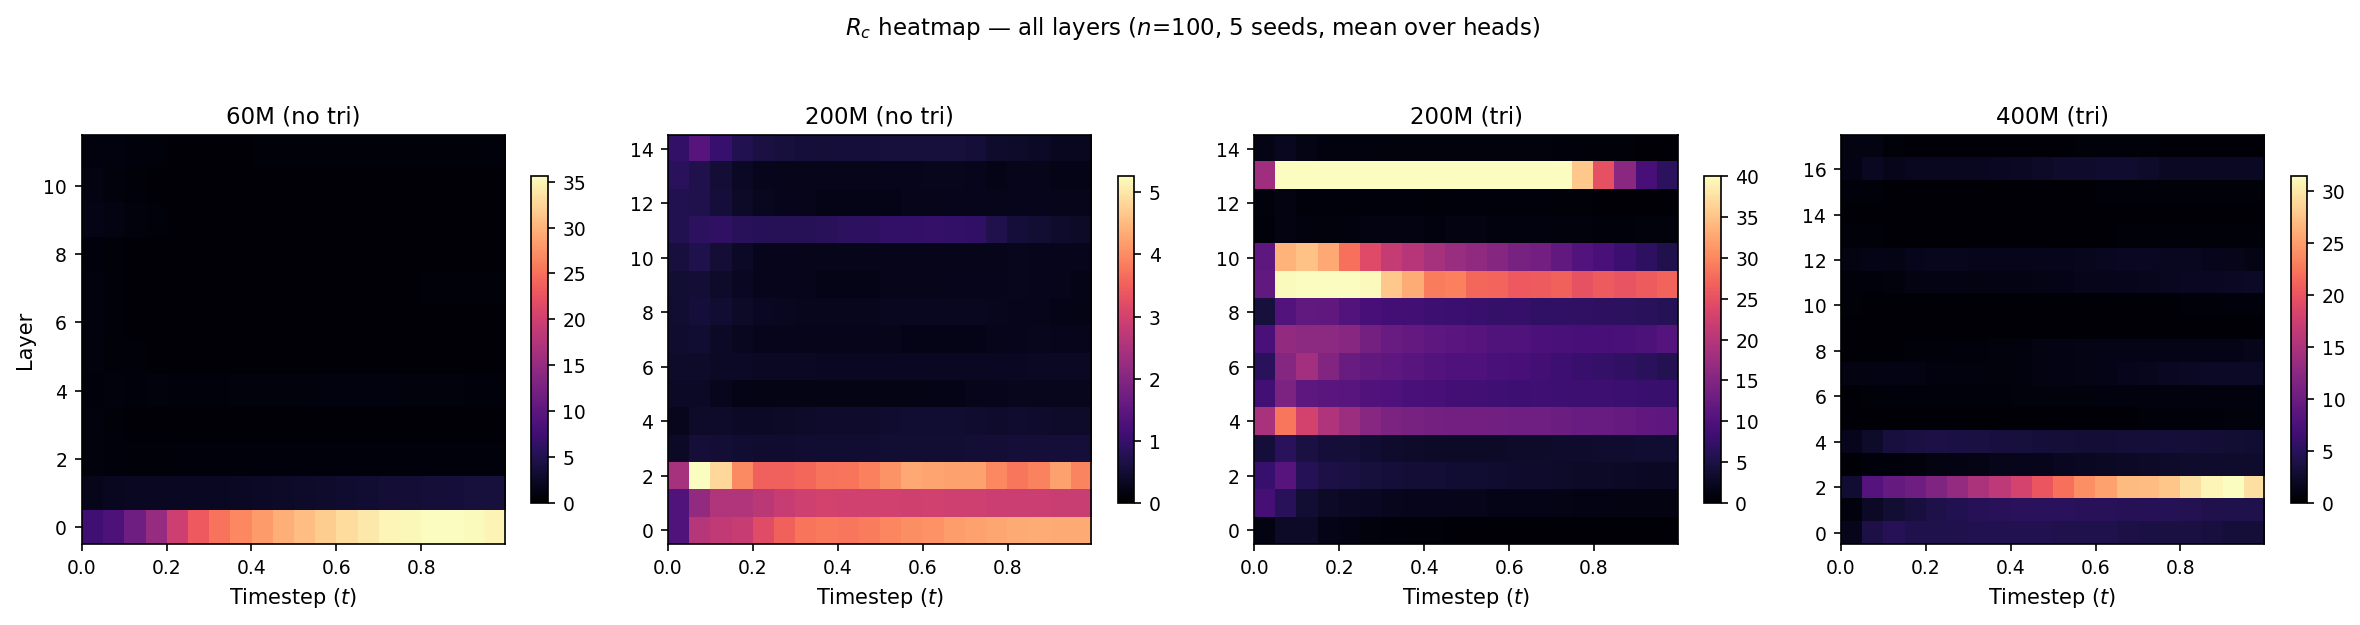
\includegraphics[width=\textwidth]{figures/fig1b-Rc-heatmaps.png}
    \caption{$R_c$ (row-centred geometry/content ratio) across all layers and timesteps (mean over heads, 5 seeds). Each model concentrates geometry dominance in a peak layer, but the location differs: L0 in 60M, L0/L2 in 200M no-tri, distributed and deep in 200M tri, L2 in 400M tri. $R_c$ grows from $t{=}0$ to $t{=}1$ in all models.}
    \label{fig:rc_heatmaps}
\end{figure}

\begin{figure}[t]
    \centering
    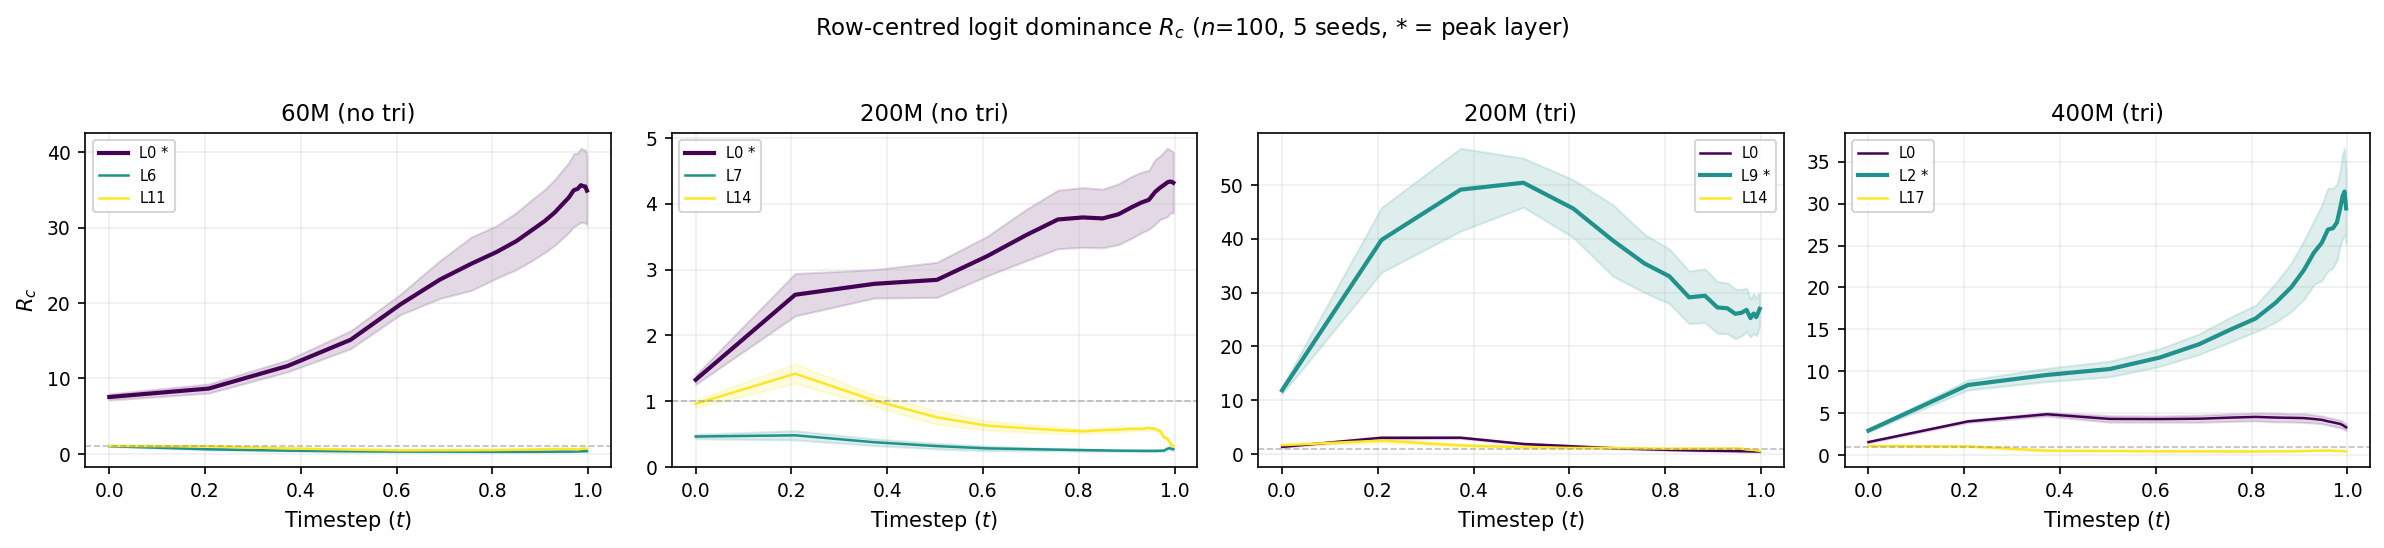
\includegraphics[width=\textwidth]{figures/fig1a-Rc-lines.png}
    \caption{$R_c$ for key layers over generation time ($n{=}100$, 5 seeds). Peak $R_c$ layer marked with $*$. Dashed line: $R_c = 1$ (balanced). Geometry increasingly dominates content at late $t$, but this varies by layer and model.}
    \label{fig:rc_lines}
\end{figure}

% ============================================================
\subsection{Causal: The Present Is Sufficient and History Is Irrelevant}
\label{sec:causal}

Having characterised where $B$ dominates descriptively, we ask when and where it must be present (results summarised in Table~\ref{tab:ablation}).

\begin{table}[t]
    \centering
    \footnotesize
    \setlength{\tabcolsep}{3.5pt}
    \caption{Structural quality under bias ablation ($n{=}100$, 3 seeds). Temporal asymmetry is universal; spatial sensitivity is architecture-dependent. $R_g$ and Cl are means across 3 seeds (1 independently generated structure per seed). \textsuperscript{\S}Deep-only $B$: $B$ active in L6--11 (60M), L8--14 (200M), L10--17 (400M). \textsuperscript{\textdagger}Shallow-only $B$: $B$ active in L0--5 (60M), L0--7 (200M), L0--9 (400M tri). \textsuperscript{\ddag}Peak-$R_c$: L0 (60M), L2 (200M no-tri), L9 (200M tri), L2 (400M tri). The single clash in the 400M tri baseline reflects one steric contact across the 3 seeds; this is within the normal variation of valid protein backbones.}
    \label{tab:ablation}
    \begin{tabular}{lcccccccc}
        \toprule
        & \multicolumn{2}{c}{\textbf{60M no-tri}} & \multicolumn{2}{c}{\textbf{200M no-tri}} & \multicolumn{2}{c}{\textbf{200M tri}} & \multicolumn{2}{c}{\textbf{400M tri}} \\
        \cmidrule(lr){2-3} \cmidrule(lr){4-5} \cmidrule(lr){6-7} \cmidrule(lr){8-9}
        Condition & $R_g$ & Cl & $R_g$ & Cl & $R_g$ & Cl & $R_g$ & Cl \\
        \midrule
        \multicolumn{9}{l}{\emph{Reference}} \\[2pt]
        Baseline & 1.44 & 0 & 1.36 & 0 & 1.42 & 0 & 1.27 & 1 \\
        Full ablation ($B{=}0$) & 0.12 & 3532 & 0.14 & 2968 & 0.07 & 4702 & 0.11 & 4021 \\
        Random $B$ $[\mathcal{N}(0,\sigma_B^2)]$ & 0.10 & 4181 & 0.18 & 1861 & 0.08 & 4648 & 0.12 & 3675 \\
        \midrule
        \multicolumn{9}{l}{\emph{Temporal}} \\[2pt]
        Early-only $B$ ($t{\leq}0.5$) & 0.12 & 3532 & 0.14 & 2967 & 0.07 & 4702 & 0.11 & 4021 \\
        Late-only $B$ ($t{>}0.5$) & 1.19 & 0 & 1.19 & 4 & 1.12 & 2 & 1.17 & 1 \\
        \midrule
        \multicolumn{9}{l}{\emph{Spatial}} \\[2pt]
        Deep-only $B$\textsuperscript{\S} & 0.41 & 558 & 0.57 & 51 & 0.90 & 0 & 0.82 & 1 \\
        Shallow-only $B$\textsuperscript{\textdagger} & 0.60 & 23 & 0.63 & 32 & 0.05 & 4752 & 0.12 & 3560 \\
        Peak-$R_c$ layer\textsuperscript{\ddag} & 0.81 & 1 & 1.28 & 1 & 1.17 & 1 & 1.13 & 1 \\
        \bottomrule
    \end{tabular}
\end{table}

\textbf{$B$ is causally essential and its geometric content is necessary.}
Full removal of $B$ is catastrophic in every model: $R_g < 0.15$\,nm with thousands of steric clashes vs.\ $R_g \approx 1.3$\,nm and ${\leq}1$ clash at baseline.
Replacing $B$ with magnitude-matched Gaussian noise collapses structures equally severely, confirming the model requires $B$'s geometric \emph{content}, not merely its signal magnitude.

\textbf{The late phase matters; the early phase does not.}
In the coarse ablation (Table~\ref{tab:ablation}), providing $B$ only during early generation ($t{\leq}0.5$) is indistinguishable from full ablation in all four models; providing it only during late generation preserves valid structures.
Figure~\ref{fig:temporal_sweep} characterises this asymmetry at finer resolution. Early-only $B$ always collapses regardless of split point, while late-only $B$ preserves valid structures with quality degrading gradually as the late window shrinks.
This one-sided asymmetry holds across all model scales despite order-of-magnitude variation in descriptive $R_c$, and across protein lengths $n{=}50$--200 for the 60M no-tri model (Table~\ref{tab:multilength}); we expect it to generalise, though length-invariance was not tested for larger models.

\begin{figure}[t]
    \centering
    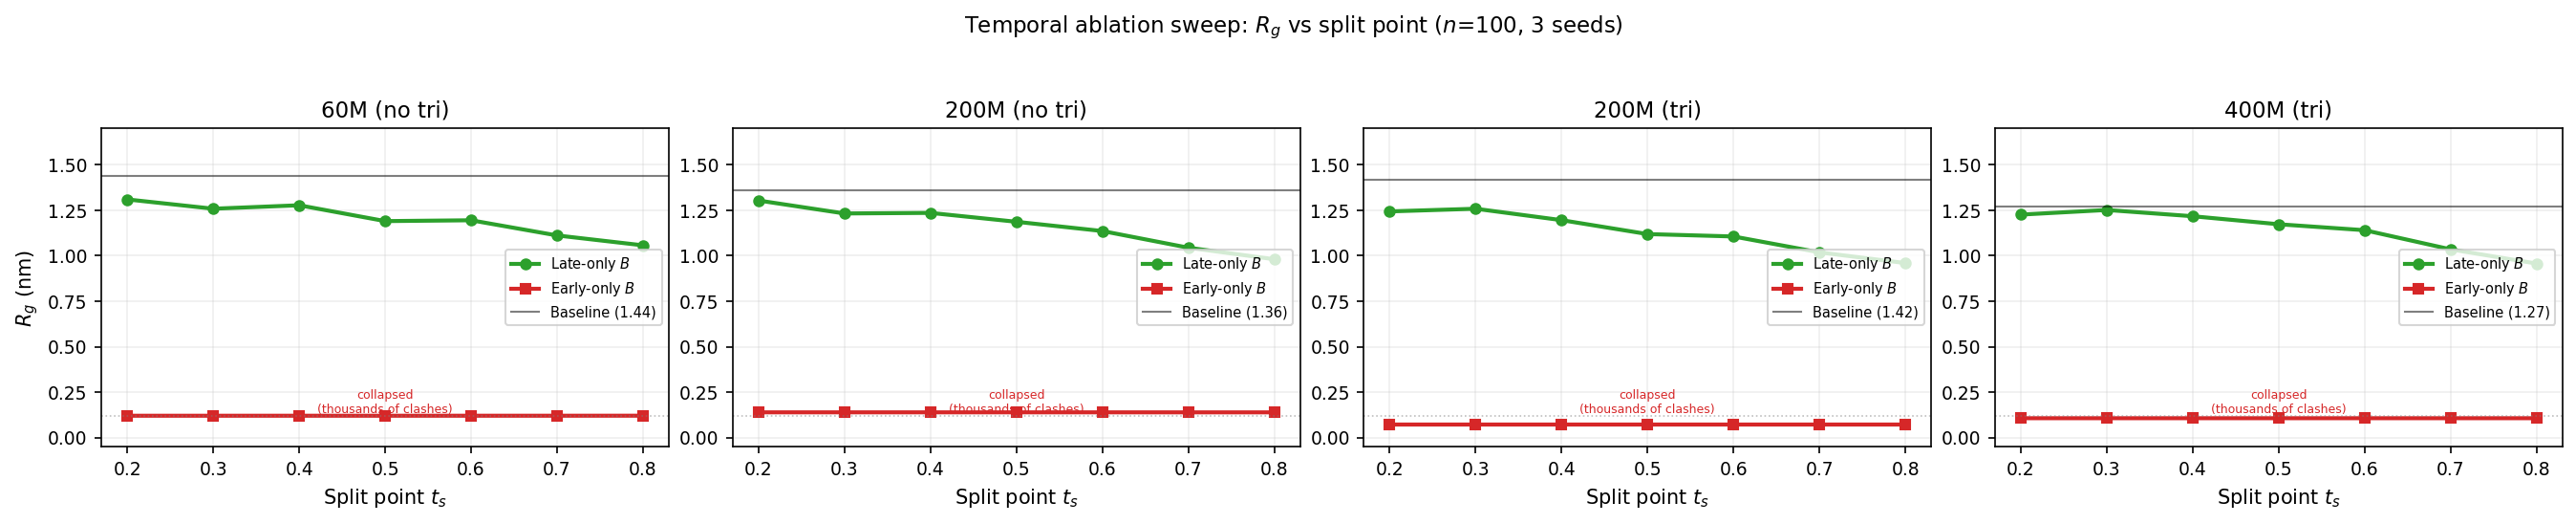
\includegraphics[width=\textwidth]{figures/fig4-temporal-sweep.png}
    \caption{Fine-grained temporal sweep ($n{=}100$, 3 seeds). Early-only $B$ (red) always collapses regardless of split point; late-only $B$ (green) always preserves valid structures. The asymmetry is one-sided and universal across all four model scales.}
    \label{fig:temporal_sweep}
\end{figure}

\textbf{The model has no memory of early $B$.}
We investigate whether this temporal asymmetry arises because early $B$ effects are transient, or because removing $B$ mid-generation causes disruption regardless of prior history.
The gap experiment tests this: $B$ is active for $t \in [0, 0.3]$, removed for $t \in (0.3, 0.7)$, then restored for $t \in [0.7, 1]$.
If removal caused active disruption, gap conditions would perform worse than late-only $B$. Instead, Table~\ref{tab:gap} shows they match within $0.02$\,nm across all four models.
A wider gap ($t \in [0, 0.2] \cup [0.8, 1]$) produces the same result: gap conditions match the corresponding late-only controls within $0.02$\,nm across all models (Table~\ref{tab:gap}).
Early $B$ leaves no lasting trace: the trajectory appears to forget both its presence and its absence.

\begin{table}[h]
    \centering
    \caption{Gap experiment ($n{=}100$, 3 seeds). Gap conditions (B on $\to$ off $\to$ on) match late-only controls within 0.02\,nm across all models. Values are means across 3 seeds (1 structure per seed).}
    \label{tab:gap}
    \begin{tabular}{lcccccccc}
        \toprule
        & \multicolumn{2}{c}{\textbf{60M no-tri}} & \multicolumn{2}{c}{\textbf{200M no-tri}} & \multicolumn{2}{c}{\textbf{200M tri}} & \multicolumn{2}{c}{\textbf{400M tri}} \\
        \cmidrule(lr){2-3} \cmidrule(lr){4-5} \cmidrule(lr){6-7} \cmidrule(lr){8-9}
        Condition & $R_g$ & Cl & $R_g$ & Cl & $R_g$ & Cl & $R_g$ & Cl \\
        \midrule
        Baseline & 1.44 & 0 & 1.36 & 0 & 1.42 & 0 & 1.27 & 1 \\
        Gap (on--off--on, 0--0.3, 0.7--1) & 1.10 & 0 & 1.04 & 3 & 1.01 & 3 & 1.05 & 1 \\
        Late-only $B$ ($t{>}0.7$) & 1.11 & 0 & 1.04 & 3 & 1.02 & 2 & 1.04 & 1 \\
        Gap (on--off--on, 0--0.2, 0.8--1) & 1.05 & 0 & 0.98 & 2 & 0.96 & 2 & 0.96 & 4 \\
        Late-only $B$ ($t{>}0.8$) & 1.06 & 0 & 0.98 & 3 & 0.96 & 3 & 0.96 & 2 \\
        \bottomrule
    \end{tabular}
\end{table}

\textbf{Spatial sensitivity depends on architecture.}
In no-tri models, removing $B$ from the first half of layers (Deep-only $B$) is more damaging than removing it from the second half (Shallow-only $B$).
In tri models, this inverts: first-half ablation (Deep-only $B$) is relatively benign ($R_g \geq 0.82$\,nm, 0--1 clashes), while second-half ablation (Shallow-only $B$) is catastrophic ($R_g \leq 0.12$\,nm, thousands of clashes).
Ablating the peak-$R_c$ layer individually produces only moderate damage ($R_g$ drops 5--18\%, structures remain valid), suggesting the geometric signal is not concentrated in a single bottleneck layer.
We did not test temporal sweeps within spatial ablation conditions, but the cross-model universality of the temporal pattern suggests it is robust to layer scope.

\begin{table}[h]
    \centering
    \caption{Length-invariance validation (60M no-tri, 3 seeds). Values are means across 3 seeds (1 structure per seed).}
    \label{tab:multilength}
    \begin{tabular}{lcccccc}
        \toprule
        & \multicolumn{2}{c}{\textbf{$n{=}50$}} & \multicolumn{2}{c}{\textbf{$n{=}100$}} & \multicolumn{2}{c}{\textbf{$n{=}200$}} \\
        \cmidrule(lr){2-3} \cmidrule(lr){4-5} \cmidrule(lr){6-7}
        Condition & $R_g$ & Cl & $R_g$ & Cl & $R_g$ & Cl \\
        \midrule
        Baseline & 1.15 & 0 & 1.44 & 0 & 1.96 & 0 \\
        Full ablation & 0.16 & 487 & 0.12 & 3532 & 0.09 & 18116 \\
        Early-only $B$ ($t{\leq}0.5$) & 0.16 & 487 & 0.12 & 3532 & 0.09 & 18117 \\
        Late-only $B$ ($t{>}0.5$) & 0.97 & 0 & 1.19 & 0 & 1.52 & 0 \\
        \bottomrule
    \end{tabular}
\end{table}

% ============================================================
\subsection{Functional: $B$ Carries the Structural Signal}
\label{sec:functional}

Figure~\ref{fig:contact} evaluates contact prediction across all four models.
At $t{=}1$, $B$-only precision is 5--20$\times$ above the random baseline; $C$-only is only 2--3$\times$ above random.

As noted in Section~\ref{sec:methods}, this comparison is partly tautological at late $t$: $B$ encodes distances and contacts are defined by distances.
The more informative finding is that $C$ never bridges the gap to $B$-only.
A plausible explanation is that, because all models were trained with $B$ present, $C$ was never pressured to encode redundant geometric features --- the persistent functional gap is a signature of this division of labour.
Whether $C$ could substitute for $B$ if trained without it remains an open question.

\begin{figure}[t]
    \centering
    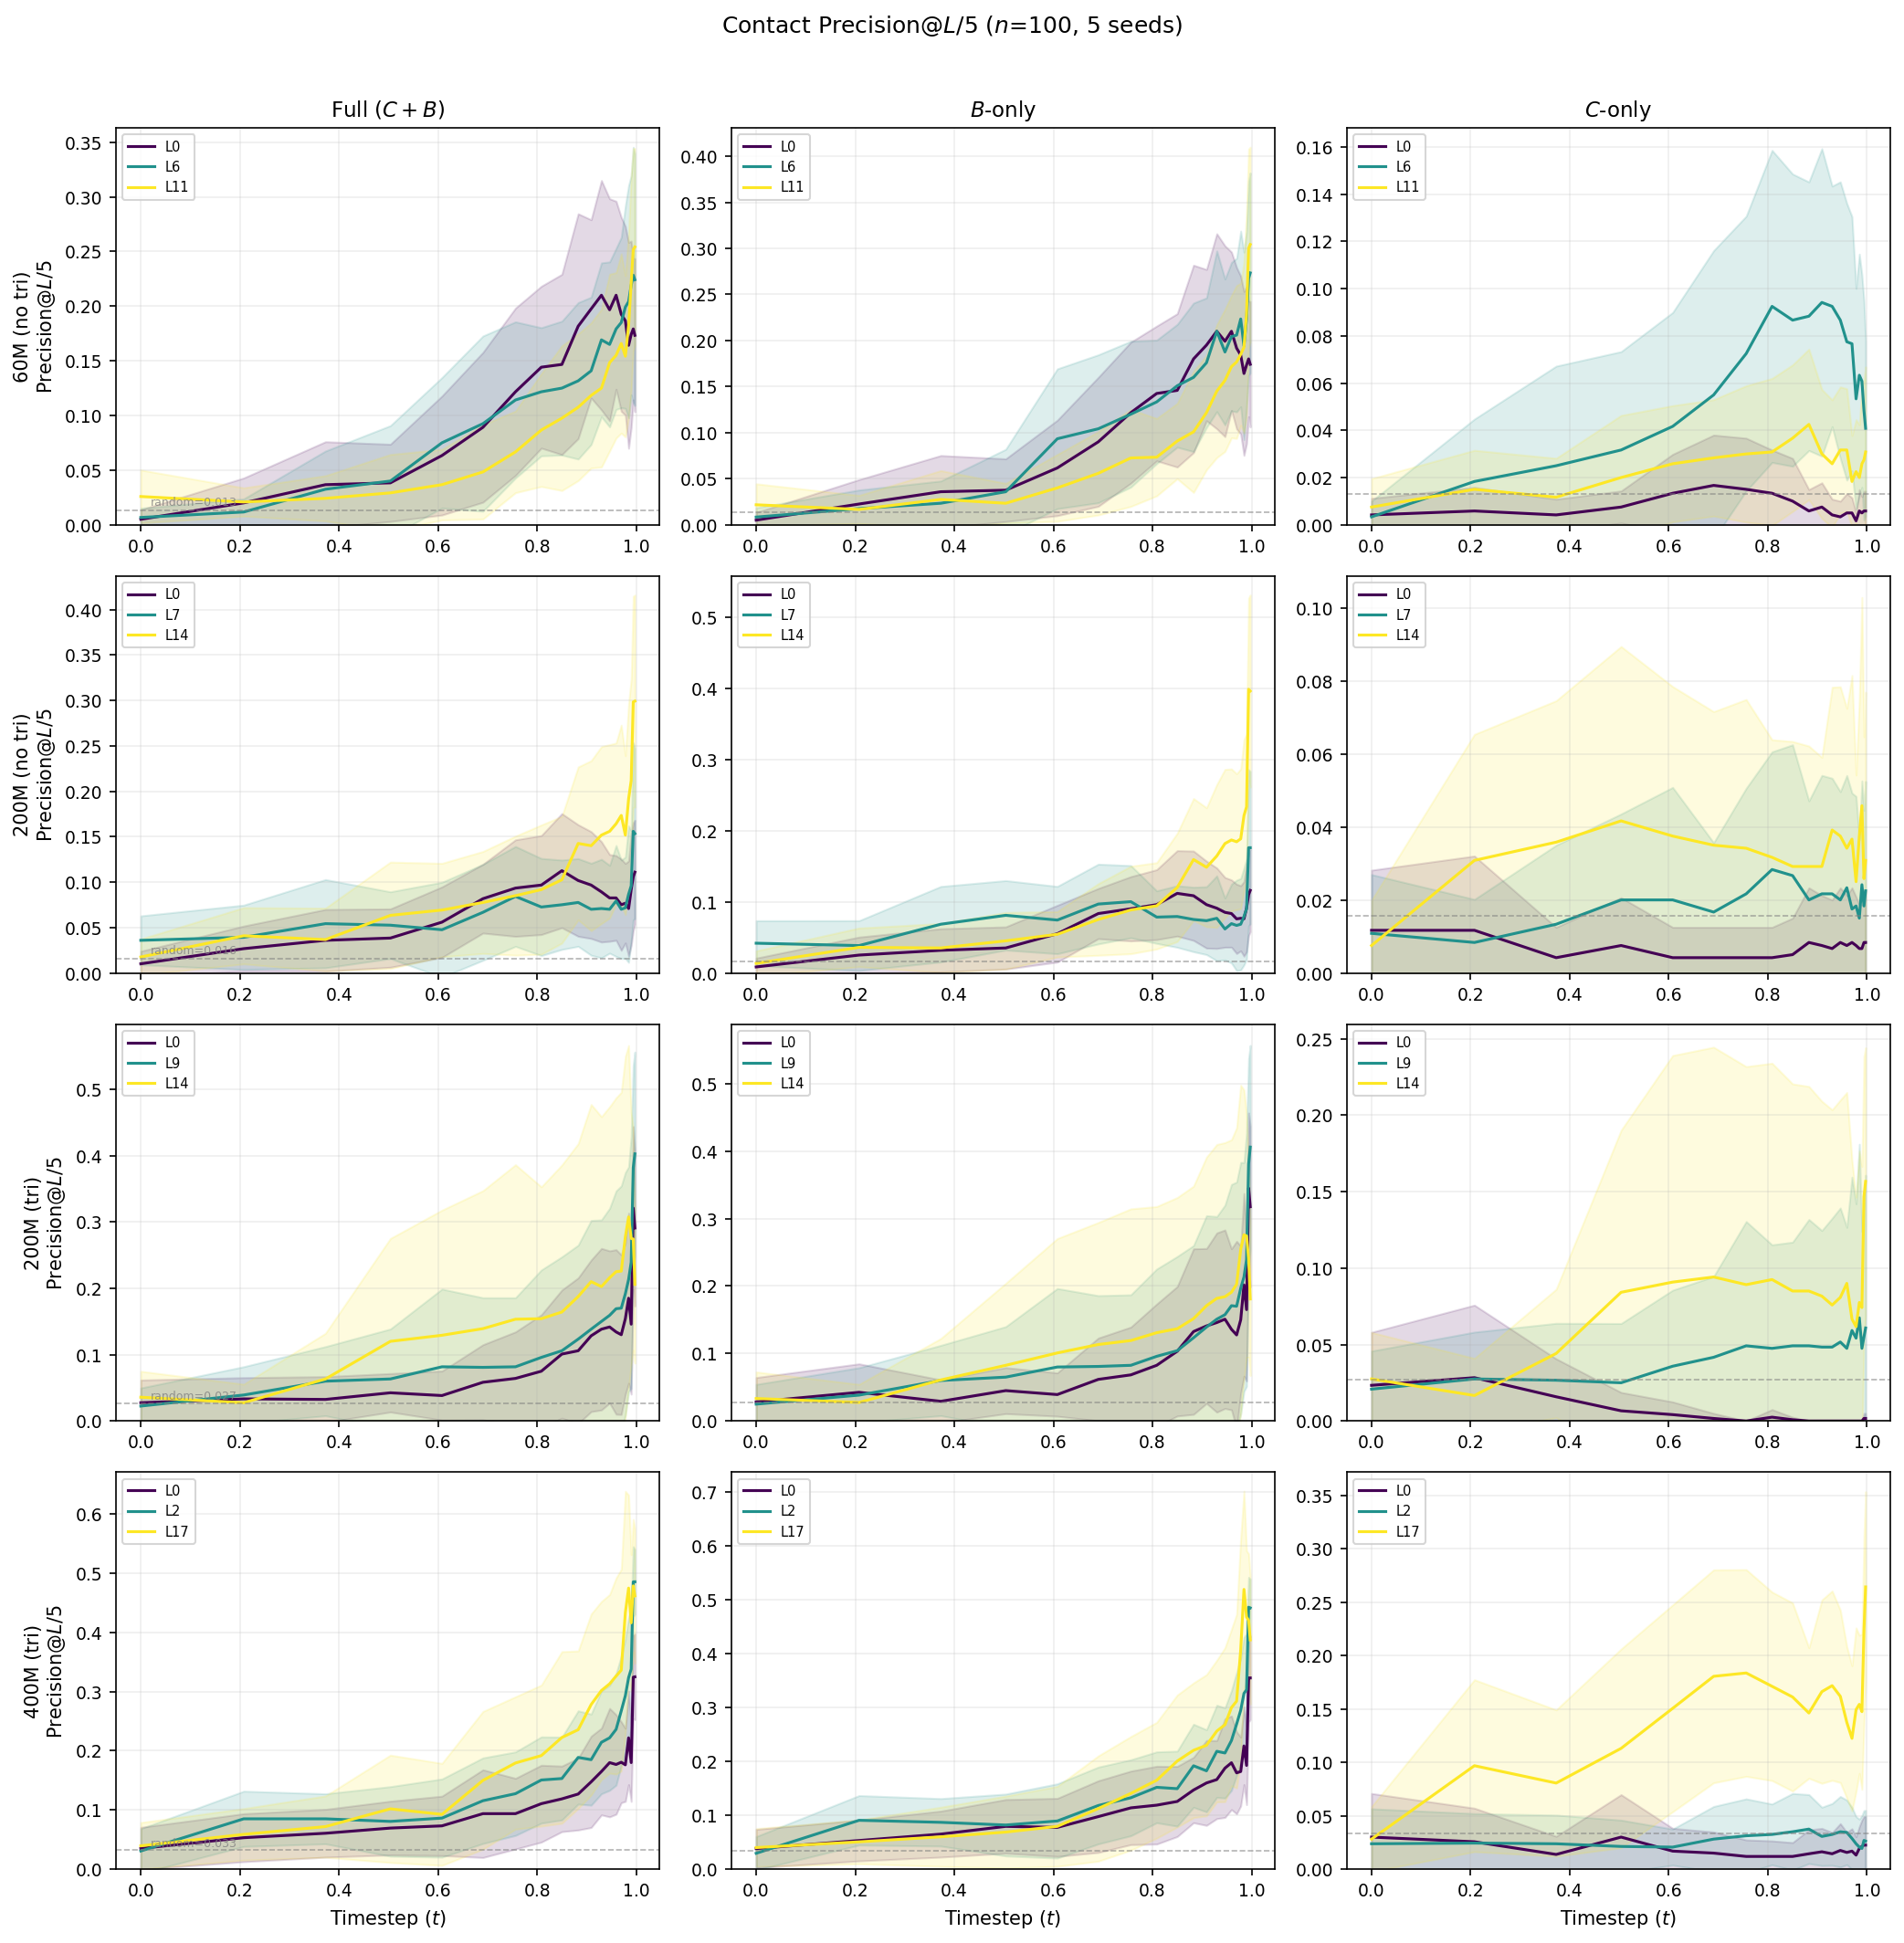
\includegraphics[width=\textwidth]{figures/fig3-contact-precision-all-models.png}
    \caption{Contact Precision@$L/5$ ($n{=}100$, 5 seeds). Dashed line: random baseline. $B$-only outperforms $C$-only at all scales, but superiority at late $t$ is partly expected by construction (see text). $C$-only never matches $B$-only, consistent with a division of labour in which $C$ does not learn to substitute for $B$.}
    \label{fig:contact}
\end{figure}

% ============================================================
\subsection{Representational: Structural Specificity Emerges Only at the Output}

Figure~\ref{fig:structurelens} applies each model's coordinate decoder to intermediate layer representations.
Contact similarity to the final output is near zero until the last 1--2 layers: intermediate representations are not in coordinate space, and structural specificity concentrates at the output.
In triangle models, RMSD decreases gradually across layers and deep layers are causally critical --- the structure lens and spatial ablation align.
In no-tri models, RMSD is uniformly high until the final layer, yet $B$ must be present in shallow layers, suggesting $B$ shapes the internal representations the final layer draws on, rather than refining a geometrically readable structure.

\begin{figure}[t]
    \centering
    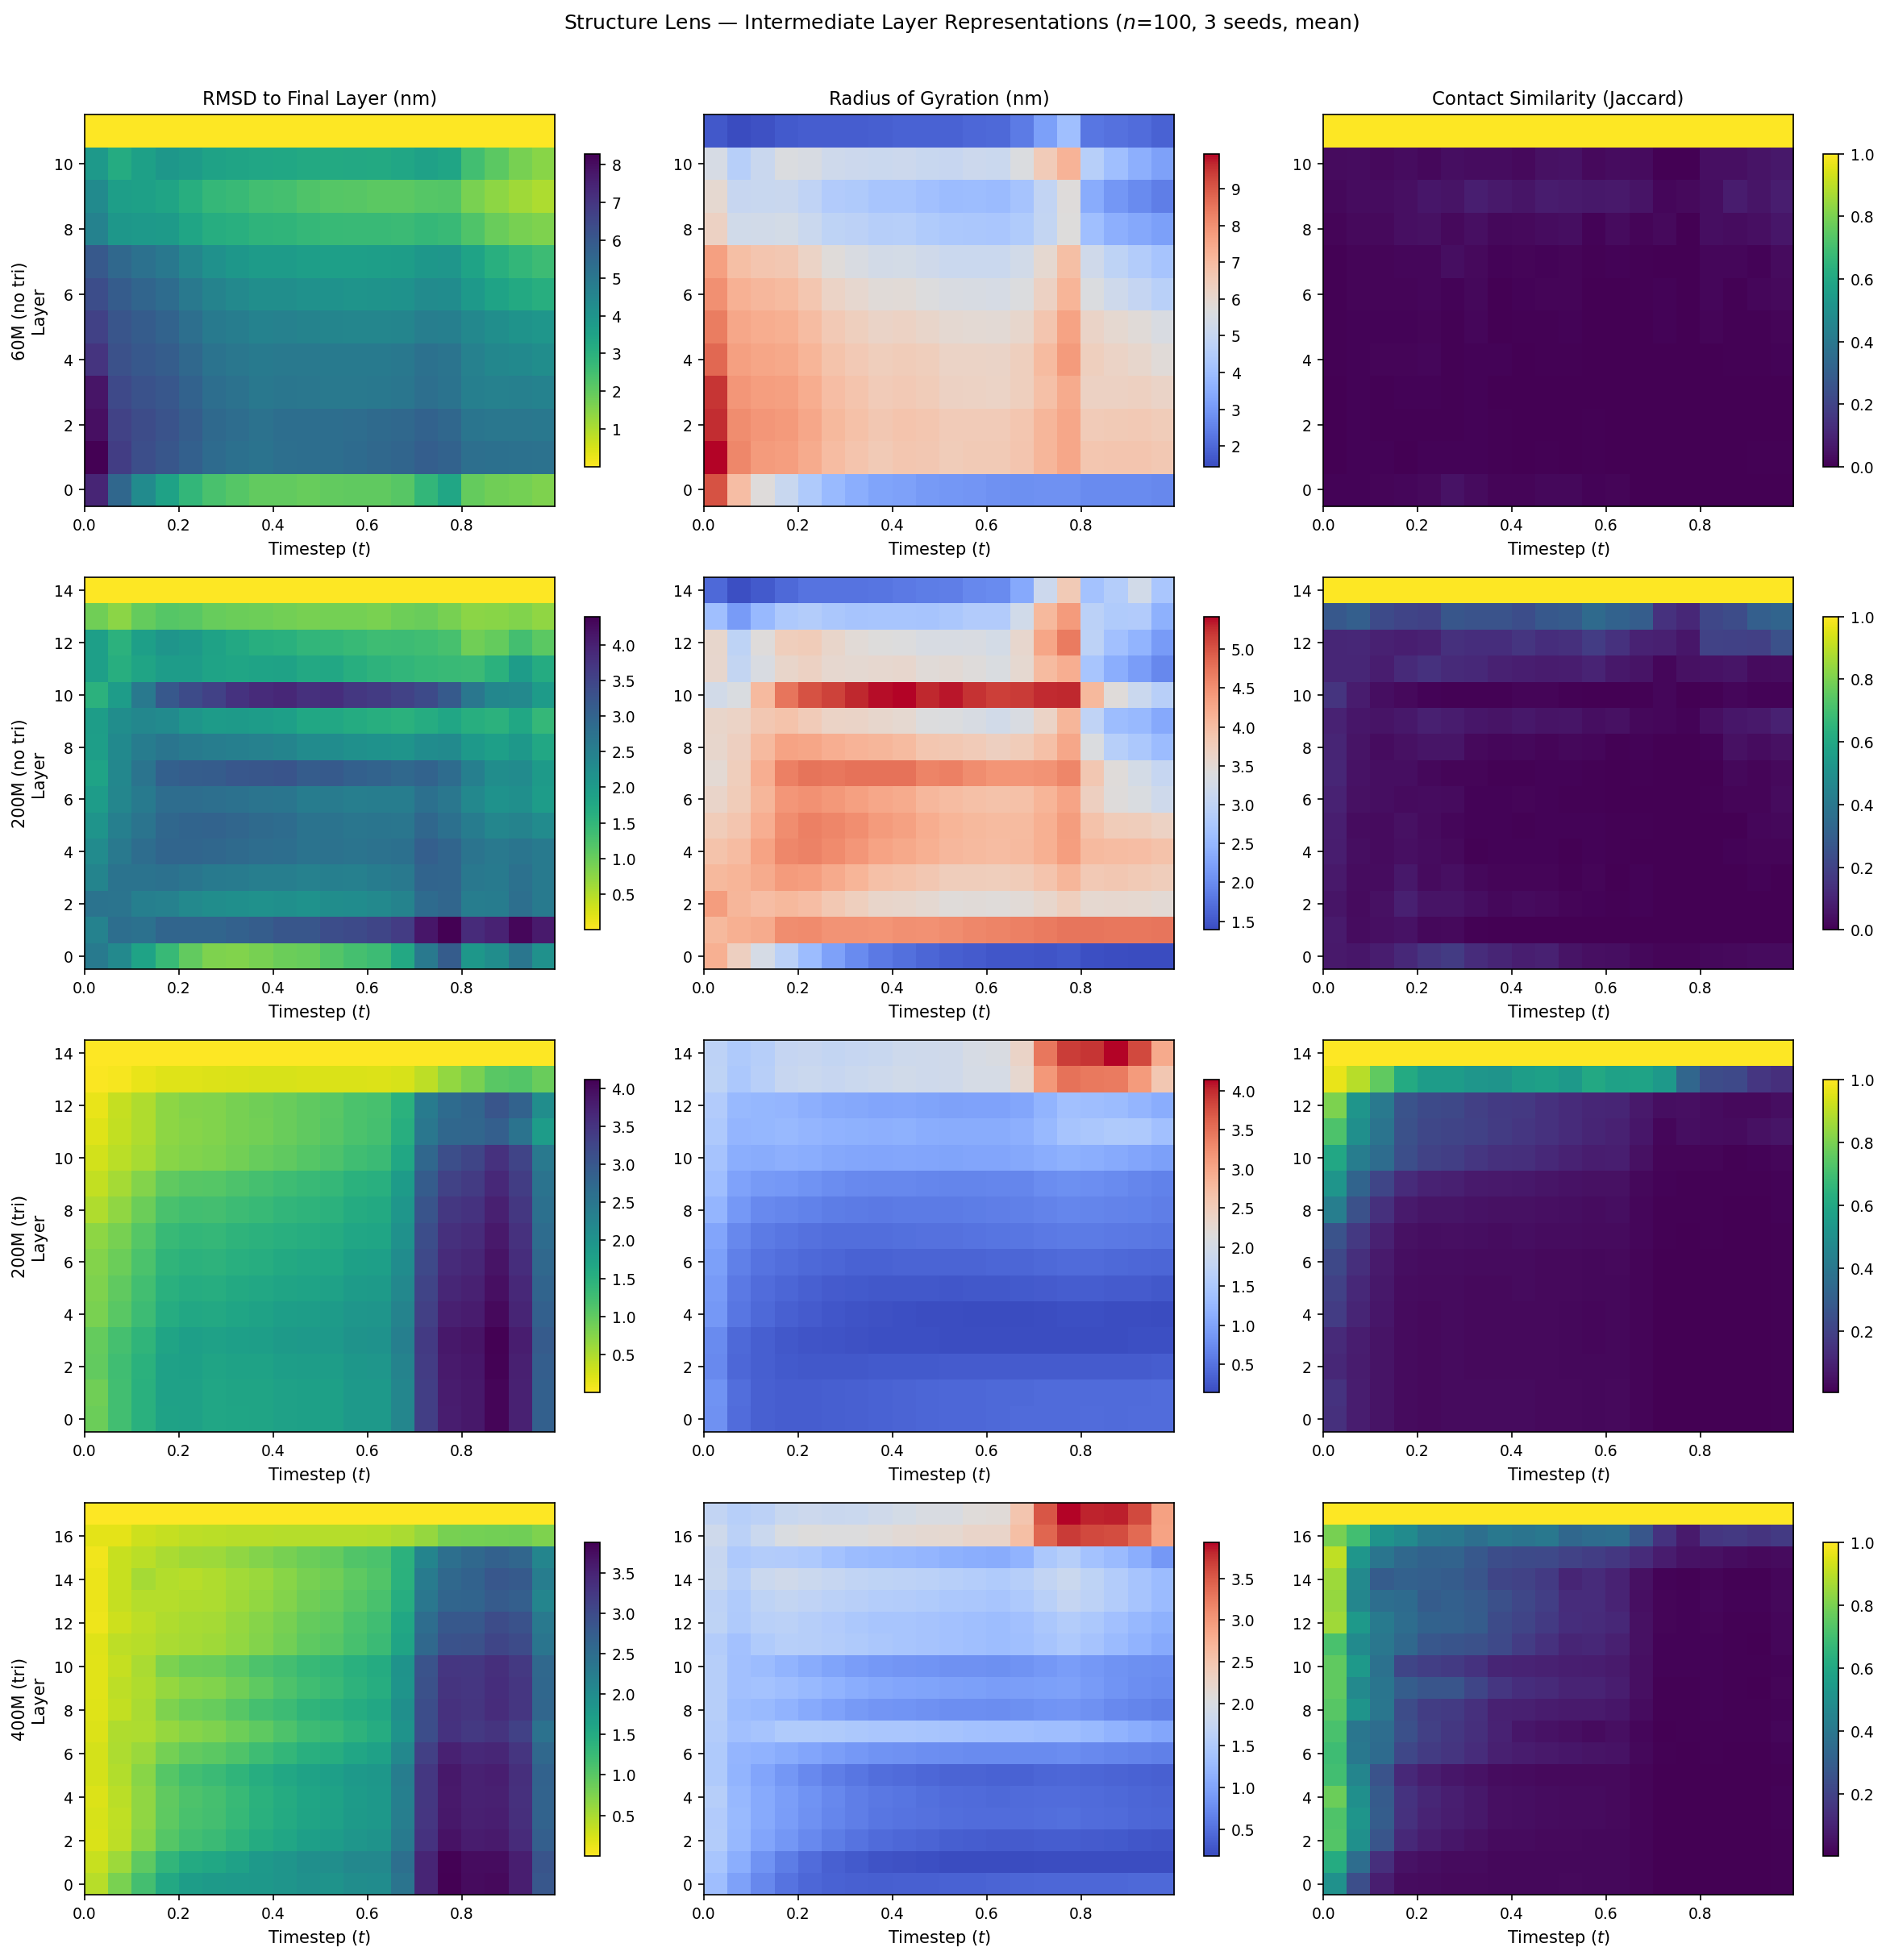
\includegraphics[width=\textwidth]{figures/fig5-structure-lens-all-models.png}
    \caption{Structure lens (3 seeds, mean). \textbf{Left:} RMSD to final-layer prediction. \textbf{Centre:} Radius of gyration. \textbf{Right:} Contact similarity (Jaccard, $<8$\,\AA, $|i{-}j|{\geq}6$). Structure specificity concentrates in the final 1--2 layers; intermediate representations are not in coordinate space.}
    \label{fig:structurelens}
\end{figure}

% ============================================================
\section{Discussion}
\label{sec:discussion}

\textbf{Geometric guidance is memoryless.}
At $t{=}0.3$, the noisy structure already has partial distance information that could provide useful coarse-grained orientation.
Yet, as the time-gap ablation shows, early $B$ leaves no trace: the model arrives at the late phase in the same representational state whether or not $B$ was present earlier.
This suggests the early-stage velocity field in the flow matching objective operates in a regime where geometric specificity is unnecessary. $B$'s role is confined to late-stage refinement when the structure is close enough to final for fine-grained geometric guidance to matter.

\textbf{Descriptive magnitude and causal necessity are decoupled.}
$R_c$ varies from 0.5 to 35 across models, and the peak layer shifts from L0 to L9. However, the temporal asymmetry is identical across all four models studied.
The 400M tri model concentrates $R_c = 29.4$ in a shallow layer, but its causal profile matches the 200M tri model in which deep layers are critical.
Signal magnitude is not a reliable proxy for causal importance; multi-lens analysis is required to avoid misleading conclusions from descriptive metrics alone.

\textbf{Limitations.}
All analyses are for unconditional generation; conditional generation may use early $B$ differently, since it encodes information from a target structure.
The functional gap between $B$-only and $C$-only contact precision may partly reflect training regime rather than an intrinsic constraint --- whether $C$ could substitute for $B$ if trained without it remains untested.
The mechanism behind the spatial inversion by triangle updates is unexplained; resolving it requires ablations separately controlling triangle update depth and $B$ ablation depth.

% ============================================================
\section{Conclusion}

Geometric pair bias in Proteina is causally dispensable during early generation and essential only during late structural refinement.
The model retains no memory of early $B$: what matters is not whether $B$ was ever present, but whether it is present \emph{now}.
Architecture changes \emph{where} this dependency is localised, but not \emph{when} it activates.

\textbf{Future work.}
If geometric guidance is actionable only in late generation, this opens the door to late-stage geometric steering --- for example, aligning intermediate representations to structure-based objectives such as atomic potentials or fold classifiers during the final denoising steps.
Conversely, early generation may benefit from content-aligned representation objectives, connecting to emerging work on representation alignment in generative models~\citep{yu2025repa}.

\bibliographystyle{unsrtnat}
\begin{thebibliography}{10}

\bibitem[Abramson et~al.(2024)]{abramson2024alphafold3}
J.~Abramson et~al.
\newblock Accurate structure prediction of biomolecular interactions with {AlphaFold} 3.
\newblock \emph{Nature}, 630:493--500, 2024.

\bibitem[Darcet et~al.(2024)]{darcet2024registers}
T.~Darcet, M.~Oquab, J.~Mairal, and P.~Bojanowski.
\newblock Vision transformers need registers.
\newblock In \emph{ICLR}, 2024.

\bibitem[Dosovitskiy et~al.(2021)]{dosovitskiy2021image}
A.~Dosovitskiy et~al.
\newblock An image is worth 16x16 words: Transformers for image recognition at scale.
\newblock In \emph{ICLR}, 2021.


\bibitem[Fuchs et~al.(2020)]{fuchs2020se3}
F.~Fuchs, D.~Worrall, V.~Fischer, and M.~Welling.
\newblock {SE(3)-Transformers}: 3{D} roto-translation equivariant attention networks.
\newblock In \emph{NeurIPS}, 2020.

\bibitem[Geffner et~al.(2025)]{geffner2025proteina}
T.~Geffner, K.~Didi, Z.~Zhang, et~al.
\newblock Proteina: Scaling flow-based protein structure generative models.
\newblock In \emph{ICLR (Oral)}, 2025.

\bibitem[Jumper et~al.(2021)]{jumper2021alphafold2}
J.~Jumper et~al.
\newblock Highly accurate protein structure prediction with {AlphaFold}.
\newblock \emph{Nature}, 596:583--589, 2021.

\bibitem[Kim et~al.(2022)]{kim2022tokengt}
J.~Kim, D.~Nguyen, S.~Min, S.~Cho, M.~Lee, H.~Lee, and S.~Hong.
\newblock Pure transformers are powerful graph learners.
\newblock In \emph{NeurIPS}, 2022.

\bibitem[Kynk\"{a}\"{a}nniemi et~al.(2024)]{kynkaanniemi2024guidance}
T.~Kynk\"{a}\"{a}nniemi, M.~Aittala, T.~Karras, S.~Laine, T.~Aila, and J.~Lehtinen.
\newblock Applying guidance in a limited interval improves sample and distribution quality in diffusion models.
\newblock In \emph{NeurIPS}, 2024.

\bibitem[Lipman et~al.(2023)]{lipman2023flow}
Y.~Lipman, R.~T.~Q. Chen, H.~Ben-Hamu, M.~Nickel, and M.~Le.
\newblock Flow matching for generative modeling.
\newblock In \emph{ICLR}, 2023.

\bibitem[nostalgebraist(2020)]{nostalgebraist2020logitlens}
nostalgebraist.
\newblock Interpreting {GPT}: the logit lens.
\newblock Blog post, 2020.

\bibitem[Rao et~al.(2021)]{rao2020transformer}
R.~Rao, J.~Meier, T.~Sercu, S.~Ovchinnikov, and A.~Rives.
\newblock Transformer protein language models are unsupervised structure learners.
\newblock In \emph{ICLR}, 2021.

\bibitem[Yu et~al.(2025)]{yu2025repa}
S.~Yu, S.~Kwak, H.~Jang, J.~Jeong, J.~Huang, J.~Shin, and S.~Xie.
\newblock Representation alignment for generation: Training diffusion transformers is easier than you think.
\newblock In \emph{ICLR}, 2025.

\bibitem[Thomas et~al.(2018)]{thomas2018tensor}
N.~Thomas, T.~Smidt, S.~Kearnes, L.~Yang, L.~Li, K.~Kohlhoff, and P.~Riley.
\newblock Tensor field networks: Rotation- and translation-equivariant neural networks for {3D} point clouds.
\newblock \emph{arXiv preprint arXiv:1802.08219}, 2018.

\end{thebibliography}

% ============================================================
% ============================================================
\appendix
\section{Raw vs.\ Row-Centred Ratio}
\label{sec:appendix_rawvsrc}

\begin{figure}[H]
    \centering
    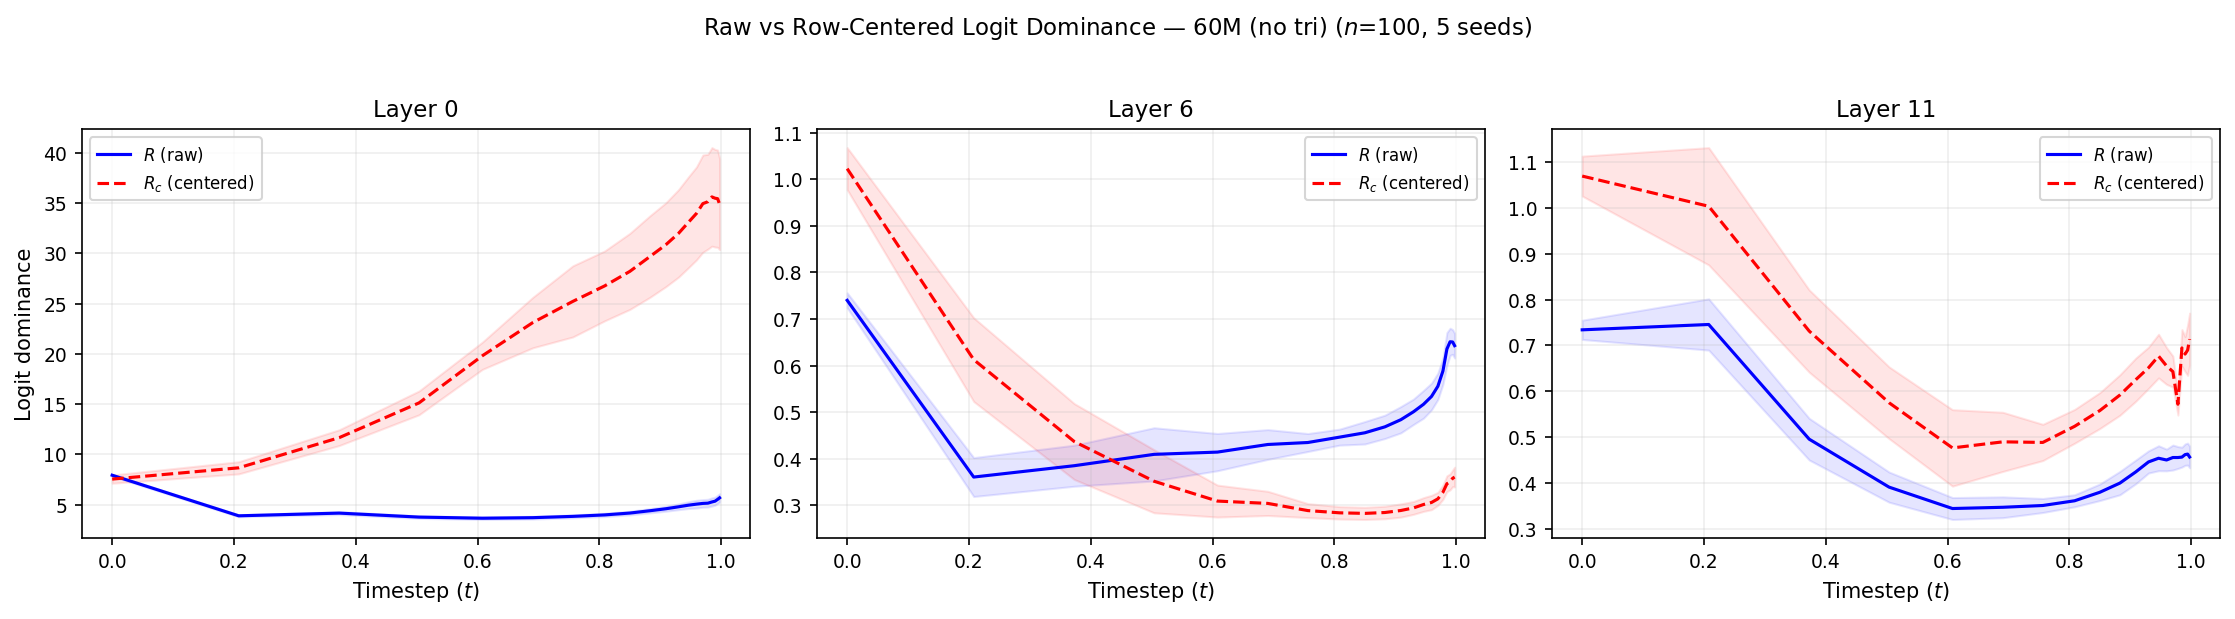
\includegraphics[width=0.7\textwidth]{figures/fig6-raw-vs-centered.png}
    \caption{Raw $R$ vs.\ row-centred $R_c$ for the 60M model. $R_c$ diverges from $R$ at late timesteps because $C$ develops large row-constant components that inflate its Frobenius norm without affecting attention. The correction reaches $6\times$ at $t{=}1$.}
    \label{fig:rawvscentered}
\end{figure}

\section{$R_c$ by Sequence Separation}
\label{sec:appendix_seqsep}

\begin{figure}[H]
    \centering
    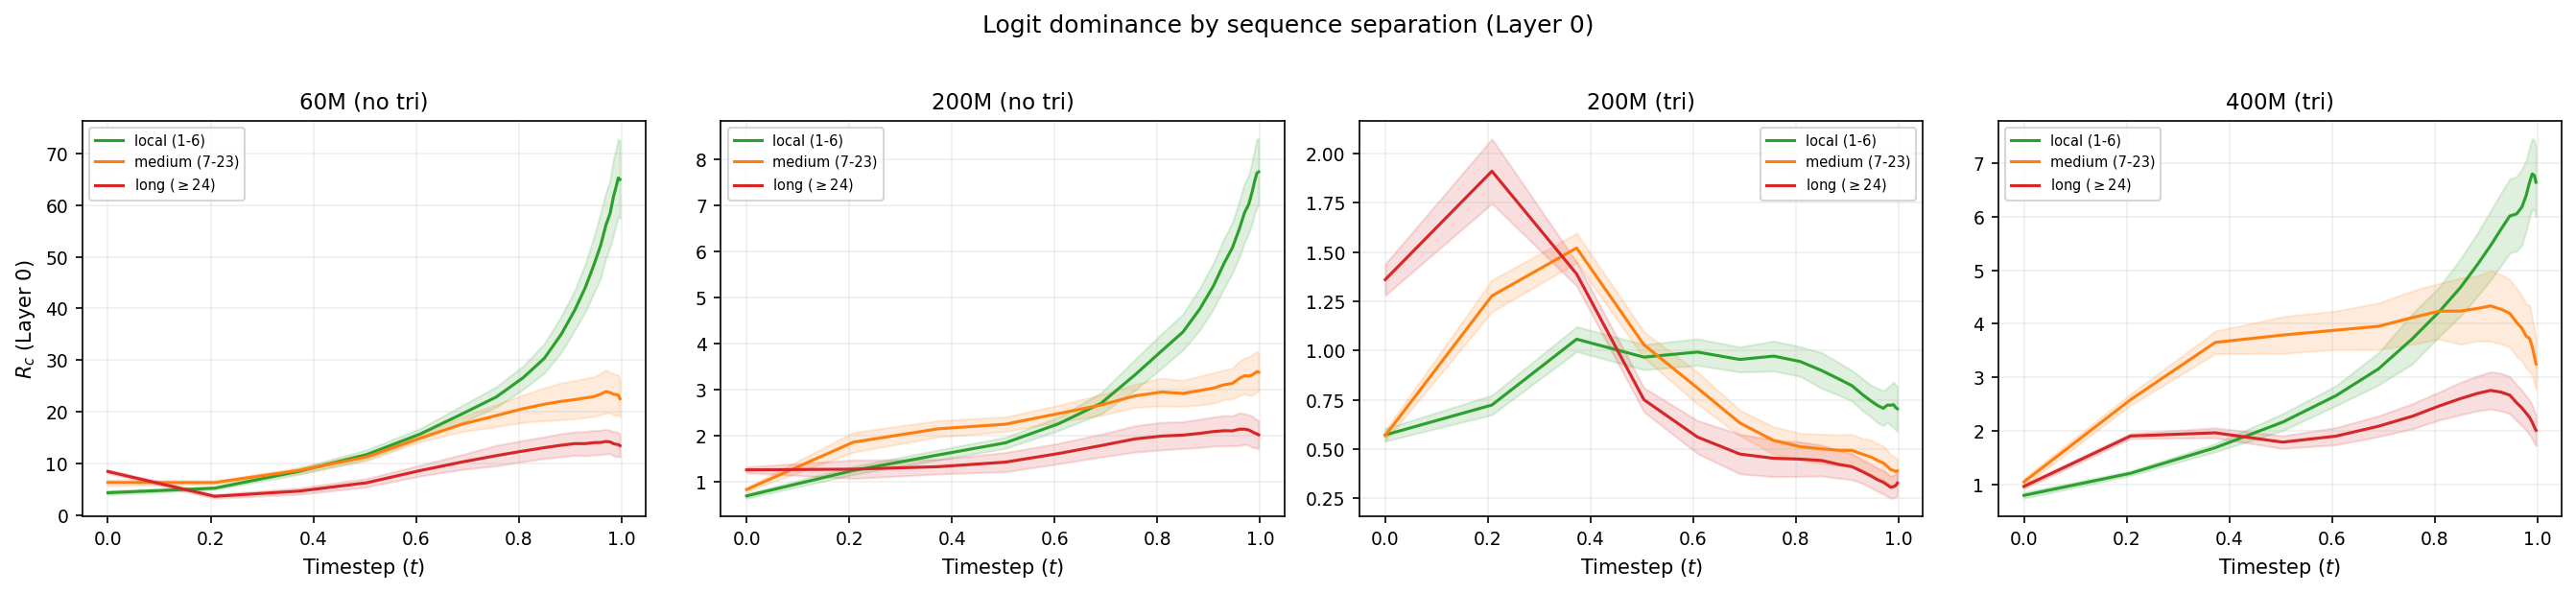
\includegraphics[width=\textwidth]{figures/fig2-seqsep-all-models.png}
    \caption{$R_c$ decomposed by residue separation in Layer~0 for all four models (5 seeds). The 60M model shows stronger range-selectivity (local vs.\ long-range pairs differ more); larger models treat pair ranges more uniformly. The 200M tri model shows a distinctive non-monotonic trajectory.}
    \label{fig:seqsep}
\end{figure}

\section{Structure Examples: Baseline vs.\ Full Ablation}
\label{sec:appendix_structures}

\begin{figure}[H]
    \centering
    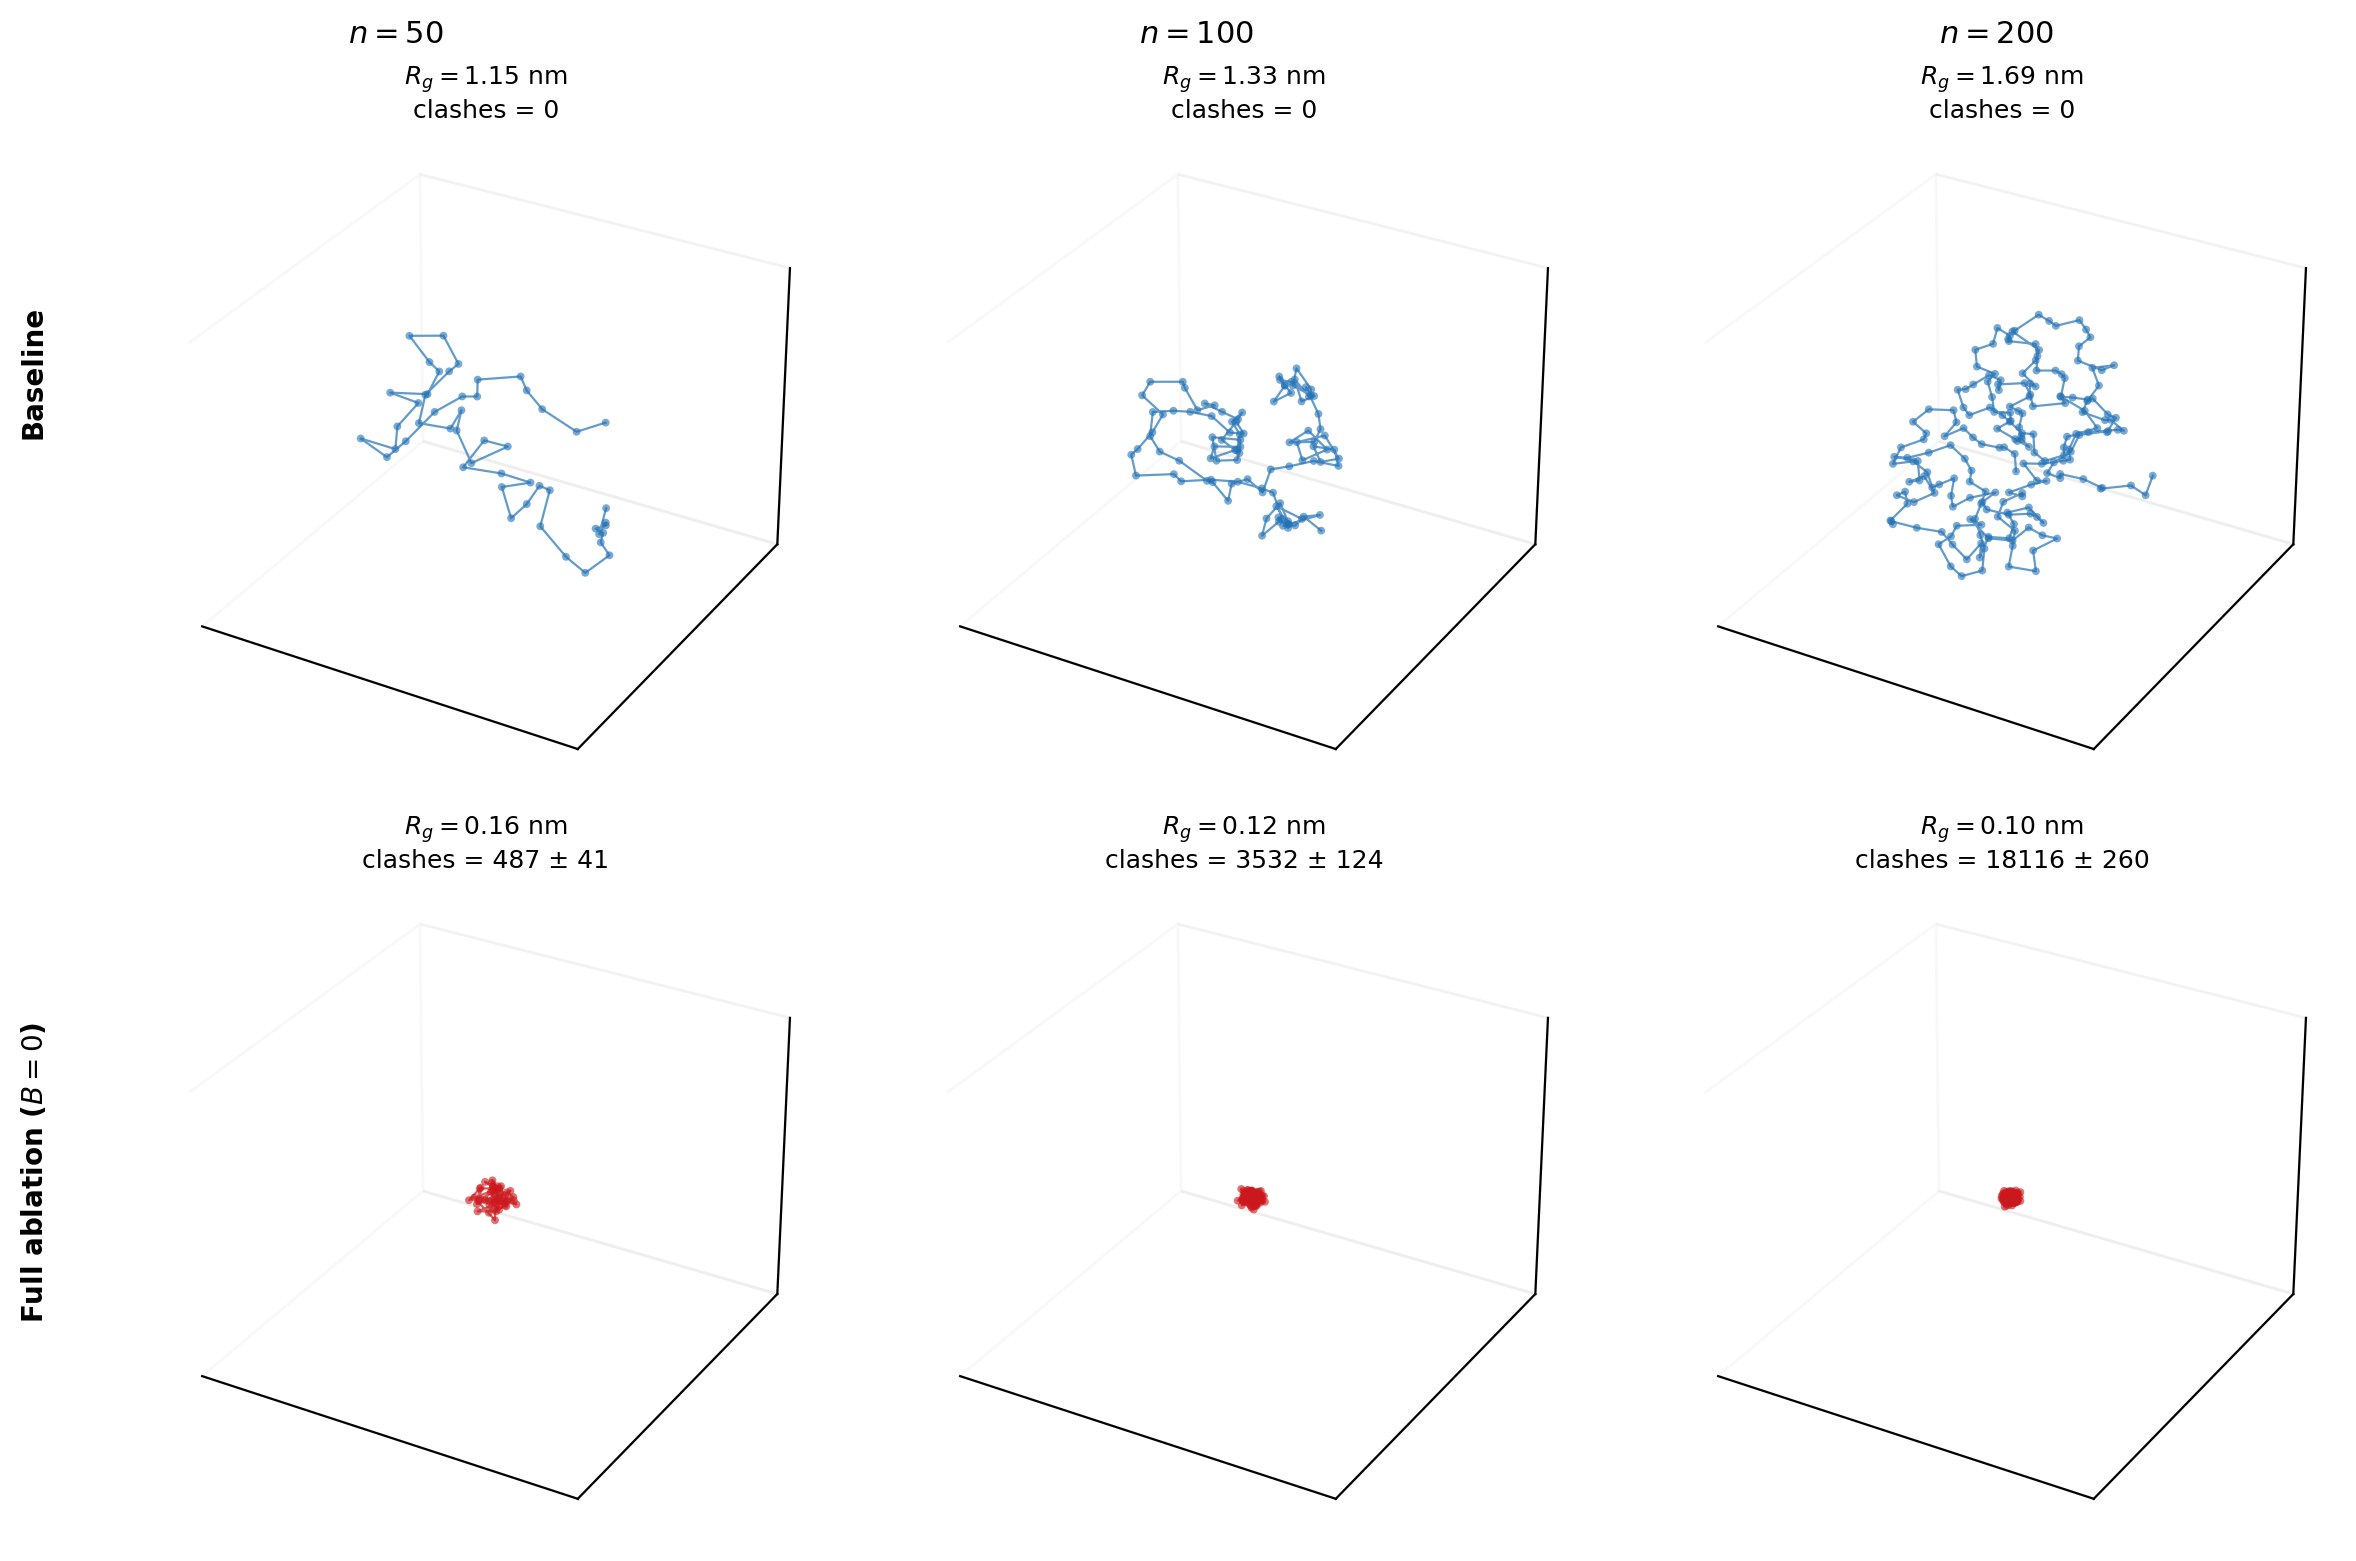
\includegraphics[width=\textwidth]{figures/figA3-structure-examples.png}
    \caption{C$\alpha$-trace renderings of three generated structures per condition (columns: $n{=}50$, $100$, $200$ residues; rows: baseline, full ablation $B{=}0$), all from the 60M model, seed 42.
    \emph{Radius of gyration} ($R_g$) measures backbone spatial spread: valid proteins have $R_g \approx 1$--$2$\,nm, while collapsed structures have $R_g < 0.2$\,nm regardless of length.
    \emph{Steric clashes} count C$\alpha$--C$\alpha$ pairs closer than the excluded-volume threshold in a single generated structure; panel titles show mean $\pm$ std across 3 independently generated structures (seeds 42, 123, 256). Baseline structures have zero clashes while fully ablated structures produce hundreds to tens of thousands.
    Each panel uses the same axis scale as the corresponding baseline panel above it, making the collapse visually apparent.}
    \label{fig:structure_examples}
\end{figure}

\end{document}
